\chapter{Background : Standard model}

\section{Elementary particle fields}
%
The \textit{standard model} (SM) of particle physics describes three fundamental interactions in nature using quantum field theory. \textit{Quantum electrodynamics} (QED) describs the electromagnetic interaction, which is responsible for attraction between electrons and neuclei in atoms and molecules. \textit{Quantum chromodynamics } (QCD) describes the strong nuclear interactions between particles. QCD is responsible for the binding of quarks inside nucleons (protons and neutrons). The weak force is behind processes such as beta decay. This weak interaction can transmute protons into neutrons, and it played a vital role in synthesizing heavy elements in the early stages of universe \cite{Barger:1987nn}. The Glashow-Weinberg-Salam (GWS) theory \cite{Glashow:1961tr, Weinberg:1967tq} pointed out that electromagnetic interaction and weak interaction can be described by a single theory, which is known as \textit{electro-weak theory}.\par
In the SM, there are matter fields and force mediating fields. The matter fields are associated with intrinsic spin $1/2$, and they are known as \textit{fermions}. Whereas force-carrying fields are associated with integer spins. These force-carrying fields are also known as \textit{gauge bosons}. \par
There are four force-carrying gauge fields in SM. The photon, which is obtained by the quantization of the electromagnetic field, mediates the electromagnetic interaction. The massive $W^{\pm}$ and $Z^{0}$ gauge bosons mediate the weak interaction. The gluons mediate the strong nuclear interactions.\par
Finally, the Higgs boson is obtained by quantizing the Higgs field.
Scalar Higgs field is involved with the mechanism that generates mass to the massive gauge bosons and matter fields except, perhaps, for neutrinos (see sec. \ref{higgssec}).\par
The fermion fields are separated into two segments, which are known as \textit{quarks} and \textit{leptons}. The quarks have six flavors, which are up ($u$), down ($d$), charm ($c$), strange ($s$), top ($t$), and bottom ($b$). There are six leptons in the lepton family. They are electron ($e$), muon ($\mu$), tau ($\tau$), electron neutrino ($v_{e}$), muon neutrino ($v_{\mu}$) and tau neutrino ($v_{\tau}$).\par
The SM elementary particle fields are summarized in figure \ref{fig:SM_summary}. 
\begin{figure}[H]
\centering
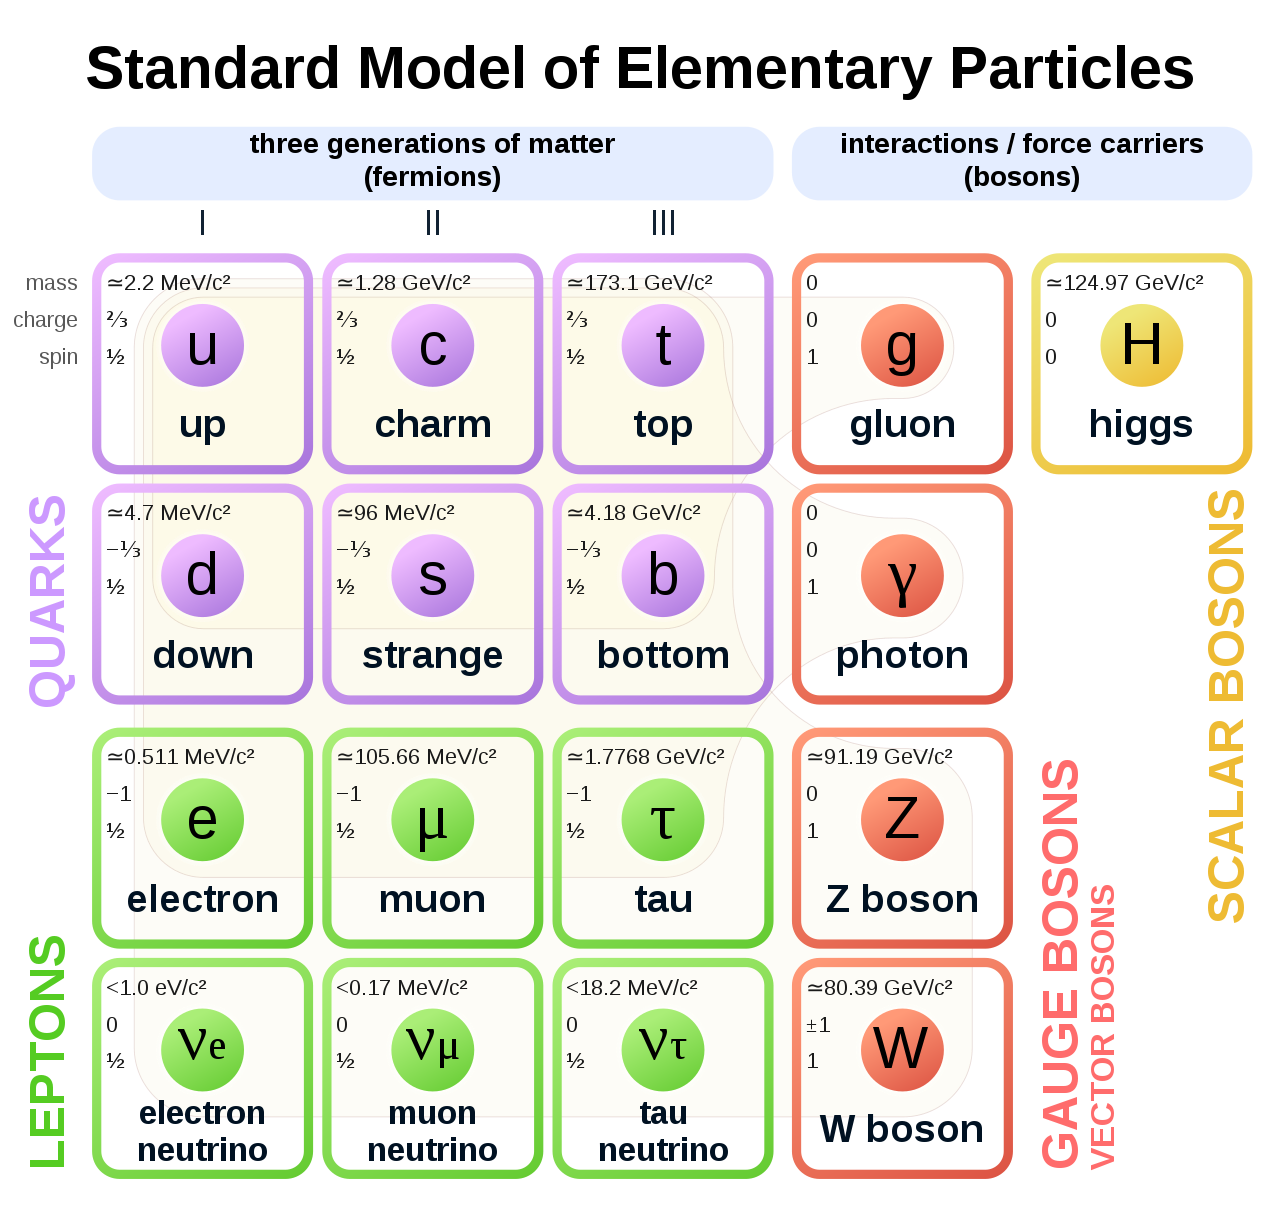
\includegraphics[width=12cm]{SM_sum.png}
\caption{\label{fig:SM_summary}
Summary of the SM elementary particles \cite{SM_summary} .}
\end{figure}
In figure \ref{fig:SM_summary}, the particles that are denoted by purple and green colors represent the matter fields. The red color represents the spin-one gauge bosons. The color yellow represents the Higgs boson. \par

\section{Symmetries in particle physics}\label{symmetry}
Symmetry transformation is an operation that can be performed on a particular system, which leaves the system invariant. The symmetries are important because they provide the conservation laws that govern the dynamics of the system. In particular, Noether's theorem connects the symmetries with the corresponding conservation laws \cite{Noether:1918zz}. For example, Noether's theorem connects the space and time translation symmetries to energy and momentum conservation, respectively \cite{Griffiths:2008zz}. \par
\subsection{Discrete symmetries}
Discrete symmetries are associated with the non-continuous change of the system. Under the discrete transformations, the system suddenly changes from one state to another. In particle physics, three important discrete symmetries govern the interactions, and they are known as \textit{parity} (P), \textit{charge conjugation} (C) and \textit{time reversal} (T).\par
The parity symmetry implies that the physical processes are invariant under flipping of the sign of space coordinates. This can be used to test whether the fundamental interactions are invariant under parity. The experimental evidence implies that the electromagnetic and strong interaction are invariant under parity. However, the weak interaction does not preserve the parity invariance \cite{Lee:1956qn}. \par
The charge conjugation transformation changes the sign of all the electromagnetic charges in the system. This implies an operator that changes the particle into an anti-particle. The strong and electromagnetic interaction both preserve charge conjugation, whereas the weak interaction does not remain invariant under C.\par
The time reversal symmetry implies that the invariance of the physical processes under the reversal of time. For example, under the T transformation a particle moving from point $A$ to $B$ along a certain path will reverse its direction from $B$ to $A$ on the same path \cite{Peccei:1998jv}. The time reversal operator is an anti-unitary operator. This means the $T$ operators act on quantum numbers as well as the operators \cite{Peskin:1995ev}, which provides
\begin{eqnarray}
T(\mathrm{c}-\text { number })\psi=(\mathrm{c}-\text { number })^{*} T\psi
\end{eqnarray}
\subsection{Continuous symmetries}
Continuous transformations gradually change the system from its original state to another. These continuous transformations play an important role in understanding elementary particle interactions. 
The elementary particle fields are defined using the complex-valued mathematical spaces. Under the continuous symmetries, the physical process remains invariant when the fields are rotated. 
For instance, electromagnetic interaction is invariant when the fields are rotated by a complex phase $e^{i\alpha}$, where $\alpha$ is a real number. This symmetry is known as $U(1)$ symmetry, and it is an abstract internal symmetry of the electromagnetic field. Similarly, the massless weak boson and fermion fields satisfy another abstract symmetry called $SU(2)_L$. These symmetries are based on the field rotations of two and three-dimensional spaces.\par
As the Yang-Mills theory \cite{Yang:1954ek} points out, the associated Lagrangian for these interacting fields should be invariant under local gauge transformations. This means the Lagrangian remains the same after an internal rotation. However, this theory seems to work well only for massless gauge fields such as photon field and gluon field. The heavy vector bosons, such as $W$ and $Z$, require another mechanism to generate their masses. For this, a scalar field called \textit{Higgs} field is employed.\par
Unlike the other fields, the lowest energy state of the Higgs field is a vacuum state (a state free of excitations) with non zero field value $v$, where $v$ is known as the vacuum expectation value (vev). Thus, the system spontaneously chooses a new vacuum. This makes the ground state only posses a subset of the symmetries of Lagrangian. This process is known as \textit{spontaneous symmetry breaking}. The broken Higgs field provide the source for the accumulation of mass for massless fermion and boson fields (see section \ref{higgssec}) \cite{Lancaster:2014pza}.\par
The standard model is specified by the special unitary group $SU(3)_c\times SU(2)_L\times U(1)_Y$. QCD has non-abelian gauge symmetry called $SU(3)_C$, the weak and electromagnetic interactions exhibit $SU(2)_L\times U(1)_Y$ symmetry.  As stipulated by the Higgs mechanism, the $SU(2)_L\times U(1)_Y$ breaks to electromagnetic subgroup $U(1)_{EM}$. The coupling for strong, weak, and electromagnetic interactions are given by $g_s$ for strong interaction, $g'$ for weak hypercharge $U(1)_Y$, and $g$ for weak isospin $SU(2)_L$. $ Y$ denotes the generator of week hypercharge, and the three generators of week isospin are given by $\tau^i$ where $i=1,2,3$. For the $SU(3)_C$, there are eight generators, which are denoted by $T^a$, where $a=1,...,8$. Since the interactions between these fields have a complex structure, it is easier to divide the SM Lagrangian into several sectors for the following analysis.

\section{Constructing the SM Lagrangian}
\subsection{The gauge sector}
The gauge field for strong interactions are given by $G_{\mu}^a$, for the $SU(2)_L$ the gauge field is given by $W_{\mu}^i$ and the gauge field for the $U(1)_Y$ is given by $B_{\mu}$. The corresponding abelian/non-abelian field strength tensors for these gauge fields are given as follows:
\begin{eqnarray}\label{GaugeFieldStreangth}
\begin{aligned} B_{\mu \nu} &=\partial_{\mu} B_{\nu}-\partial_{\nu} B_{\mu} \\ W_{\mu \nu}^{i} &=\partial_{\mu} W_{\nu}^{i}-\partial_{\nu} W_{\mu}^{i}-g \epsilon^{i j k} W_{\mu}^{j} W_{\nu}^{k} \\ G_{\mu \nu}^{a} &=\partial_{\mu} G_{\nu}^{a}-\partial_{\nu} G_{\mu}^{a}-g_{s} f^{a b c} G_{\mu}^{b} G_{\nu}^{c} \end{aligned}
\end{eqnarray}
In the SM Lagrangian gauge sector is realized as follows:
\begin{eqnarray}
\mathcal{L}_{\mathrm{gauge}}=-\frac{1}{4} B_{\mu \nu} B^{\mu \nu}-\frac{1}{4} W_{\mu \nu}^{i} W^{i, \mu \nu}-\frac{1}{4} G_{\mu \nu}^{a} G^{a, \mu \nu}
\end{eqnarray}
\subsection{The fermionic sector}
The fermionic sector contains the matter fields. Also, it exhibits the $SU(2)_L\times U(1)_Y$ symmetry, which accounts the weak and electromagnetic  interactions. There are three generations of fermions each consist of \textit{neutrino} ($v_i$) with electromagnetic charge $Q_i=0$, \textit{lepton} ($l_i$) with $Q_i=-1$, up type \textit{quark} with $Q_i=+2/3$ and down type quark with $Q_i=-1/3$. The $SU(2)_L$ determines the transformation properties of these fermion fields under weak charge. These fields are arrange as a $2\times 1$ column vector. This is known as \textbf{2} representation. For an example, $u_L$ and $d_L$ together form \textbf{2} representation of $SU(2)_L$. Similarly, $v_{eL}$ and $e_L$ also transform together to form doublet. On the other hand, right handed fields transform as singlets under $SU(2)_L$.\par
The representation of $U(1)_Y$ is the \textit{hypercharge} of the field. The hypercharge is assigned based on the final electromagnetic charge of the fermion. The representation of $SU(3)_C$ is determined by the color charge. The left and right handed quarks comes in three colors as $3\times 1$ column vector. This is the \textbf{3} representation in $SU(3)_C$. Leptons do not carry a color. They are in the singlet representation of $SU(3)_C$.
Altogether, for an example, the transformation of up type quark under $SU(3)_c\times SU(2)_L\times U(1)_Y$ is
\begin{eqnarray}
u_L\sim (3,2,\frac{1}{3})
\end{eqnarray}
The interaction between the matter and gauge fields is captured by the covariant derivative.
\begin{eqnarray}
D_{\mu}=\partial_{\mu}+i g^{\prime} B_{\mu} Y+i g W_{\mu}^{i} \tau^{i}+i g_{s} G_{\mu}^{a} T^{a}
\end{eqnarray} 
Using this the fermionic part of the standard model Langrangian can be written as:
\begin{eqnarray}
\mathcal{L}_{\text{fermionic}}=\sum_{i=1}^{3}\left(\bar{E}^i_L i \slashed{D}E_{L}^i+\bar{Q}_{L}^i i\slashed{D}Q_L^i+\bar{e}_R^i i\slashed{D}e_{R}^i+\bar{u}_R^i i\slashed{D}u_R^i+\bar{d}_R^i i\slashed{D}d_R^i\right)
\end{eqnarray}
where 
\begin{eqnarray}
\begin{aligned} E_{L}^{i} &=P_{L}\left(\begin{array}{c}{\nu_{i}} \\ {e_{i}}\end{array}\right)=\left(\left(\begin{array}{c}{\nu_{e}} \\ {e}\end{array}\right)_{L},\left(\begin{array}{c}{\nu_{\mu}} \\ {\mu}\end{array}\right)_{L},\left(\begin{array}{c}{\nu_{\tau}} \\ {\tau}\end{array}\right)_{L}\right) \\ Q_{L} &=P_{L}\left(\begin{array}{c}{u_{i}} \\ {d_{i}}\end{array}\right)=\left(\left(\begin{array}{c}{u} \\ {d}\end{array}\right)_{L},\left(\begin{array}{c}{c} \\ {s}\end{array}\right)_{L},\left(\begin{array}{c}{t} \\ {b}\end{array}\right)_{L}\right), \end{aligned}
\end{eqnarray}
$P_{L / R}=\left(1 \mp \gamma^{5}\right) / 2$.\\
%Lagrangian density can be devided into couple of sections as follows.
\subsection{Higgs sector}\label{higgssec}
As discussed in the section \ref{symmetry}, the Higgs field is needed as a mass generating mechanism to heavy vector bosons. The Lagrangian is \cite{Manohar:2000dt, Lancaster:2014pza, LlewellynSmith:1973yud}: 
\begin{eqnarray}\label{higgsLagrangian}
\mathcal{L}_{\mathrm{H}}=\left(D_{\mu} \phi\right)^{\dagger}\left(D^{\mu} \phi\right)+\frac{1}{2}\mu^{2} \phi^{\dagger} \phi-\frac{1}{4}\lambda\left(\phi^{\dagger} \phi\right)^{2}+\mathcal{L}_{gauge}
\end{eqnarray}
where 
\begin{eqnarray}
\langle\phi\rangle=\left(\begin{array}{l}{\phi^+} \\ {\phi^0}\end{array}\right)=\frac{1}{\sqrt{2}}\left(\begin{array}{l}{\phi_3+i\phi_4} \\ {\phi_1+i\phi_2}\end{array}\right)
\end{eqnarray}
Here $\mu$ and $\lambda$ are both real parameters. However, the minimum of the Higgs potential is not at $\langle\phi\rangle=0$. Thus, the  potential term provides the spherical shell of minima at a radius $v=\left(\frac{\mu^2}{\lambda}\right)^{\frac{1}{2}}$. On the surface of this spherical shell there are infinitely many equivalent vacua. The Higgs field spontaneously pick one of these vacua and breaks the symmetry. For simplicity, consider the following vacuum field configuration:
\begin{eqnarray}
(\phi_1^0)^2=\frac{2\mu^2}{\lambda}=2 v^2, \text{  } \phi_2^0=0\text{  }\phi_3^0=0\text{  }\phi_4^0=0
\end{eqnarray}
More concisely, 
\begin{eqnarray}\label{higgsvcuum}
\langle\phi\rangle=\left(\begin{array}{l}{0} \\ {v}\end{array}\right)
\end{eqnarray}
The symmetry breaking $SU(2)_L\times U(1)_Y\rightarrow U(1)_Q$ does not break all the symmetries. For instance, our choice of vacuum given in equation (\ref{higgsvcuum}) is still invariant under $\hat{U}=e^{i(\frac{Y}{2}+I_3\tau^3)\alpha(x)}$ transformation. In fact $Q=\frac{Y}{2}+I_3$ where $Q$ is the electromagnetic charge. Using this the above transformation can be written as  $\hat{U}=e^{iQ\alpha(x)}$. According to the \textit{Yang-Mills} theory this is equivalent to a U(1) transformation. Therefore, the electromagnetic interaction emerges unbroken from this symmetry breaking. \par
The excitation above the vacuum state of the Higgs field is given below:
\begin{eqnarray}
\phi(x)=\left(\begin{array}{l}{\quad 0} \\ {v+\frac{h(x)}{\sqrt{2}}}\end{array}\right)
\end{eqnarray}
The first term in the Higgs Lagrangian becomes
\begin{eqnarray}
(D_{\mu}^{\dagger}\phi)(D^{\mu}\phi)=\frac{1}{2}(\partial_{\mu}h(x))^2+\frac{g^2v^2}{4}(W_{\mu}^1)^2+\frac{g^2v^2}{4}(W^2_{\mu})^2+\frac{v^2}{4}(g W_{\mu}^3-g'B_{\mu})^2
\end{eqnarray}
Note that the mass term of a spin-1 field has the form $\frac{1}{2}(mass)^2\times(field)^2$. Following from this, the $W_{\mu}^1$ and $W_{\mu}^2$ fields obtain a mass $M^2_W=\frac{g^2v^2}{2}$. The linear combination of the fields $(g W_{\mu}^3-g'B_{\mu})$ also becomes massive. The Higgs field components $\phi_2,\phi_3$ and $\phi_4$ disappeared from the interaction Lagrangian. The massive excitation of the scalar field is known as \textit{Higgs} boson.\par
The linear combination $g'W^3_{\mu}+gB_{\mu}$ does not appear in the above Lagrangian. Therefore, this combination is identified as the massless photon field. The \textit{Weinberg angle} is defined as the ratio of coupling constants $g$ and $g'$ as $\tan \theta_W=\frac{g'}{g}$. Using this angle two new fields are defined as:
\begin{eqnarray}
\left(\begin{array}{l}{Z_{\mu}} \\ {A_{\mu}}\end{array}\right)=\begin{pmatrix} 
\cos\theta_W & -\sin\theta_W \\
\sin\theta_W & \cos\theta_W 
\end{pmatrix}\left(\begin{array}{l}{W_{\mu}^3} \\ {B_{\mu}}\end{array}\right)
\end{eqnarray}  
where $Z_{\mu}$ is the $Z$ boson field and $A_{\mu}$ is the photon field.
\subsection{Yukawa sector}
The Higgs couplings to the fermions in the SM is described by the \textit{Yukawa} Lagrangian. The Lagrangian needs to be \textit{Lorentz invariant} and have mass dimension 4. Its general form is
\begin{eqnarray}
\mathcal{L}_{\mathrm{Yukawa}} \ni -y_{\psi}\bar{\psi}_R\phi\psi_L+ \mbox{c.c},
\end{eqnarray} 
where $\psi$ and $\phi$ are fermion field and scalar field respectively. $y_{\psi}$ is the dimensionless coupling between the scalar and fermion fields, which is known as the \textit{Yukawa coupling}.
\subsubsection{Lepton sector}
\vspace{-0.3cm}
Using the above definition, the Yukawa term in the Lagrangian can be obtained for the $SU(2)_L$ doublet $E_{L}=\left(\nu_{L}, e_{L}\right)^{T}$ as follows:
\begin{eqnarray}
\mathcal{L}_{\mathrm{Yukawa}} \ni-\left[y_{e} \overline{e}_{R} \Phi^{\dagger} E_{L}+y_{e}^{*} \overline{E}_{L} \Phi e_{R}\right]
\end{eqnarray}
The coupling $y_{e}$ is obtained using
\begin{eqnarray}
\frac{y_{e}}{\sqrt{2}}=\frac{m_{e}}{v}
\end{eqnarray} 	
Also, this can be extended to all three generations in SM. This gives a generalized lepton sector as
\begin{eqnarray}
\mathcal{L}_{\mathrm{lepton}} \ni -\left[Y_{ij} \overline{e}_{Rj} \Phi^{\dagger} E_{Li}+Y_{ij}^{*} \overline{E}_{Li} \Phi e_{Rj}\right],
\end{eqnarray} 
where $Y_{ij}$ is the matrix element of the Yukawa matrix.
Due to the absence of $\nu_{Ri}$ fields, in SM $neutrinos$ do not couple to Higgs field. The neutrinos do not get their mass from the Higgs mechanism.
\vspace{-0.3cm}
\subsubsection{Quark sector}
\vspace{-0.3cm}
Similarly, the Yukawa interaction between $SU(2)_L$ quark doublet $Q_L=\left(u_{L}, d_{L}\right)^{T}$ and down type quark singlet $d_R$ can be written as 
\begin{eqnarray}\label{downType}
\mathcal{L}_{\mathrm{Yukawa}} \ni-\left[y_{d} \overline{d}_{R} \Phi^{\dagger} Q_{L}+y_{d}^{*} \overline{Q}_{L} \Phi d_{R}\right]
\end{eqnarray}
The mass generation of up type quarks is obtained by using the conjugate doublet transformation in $SU(2)$. The conjugate Higgs doublet is given by
\begin{eqnarray}
\tilde{\phi} \equiv i \sigma^{2} \phi^{*}=i\left(\begin{array}{cc}{0} & {-i} \\ {i} & {0}\end{array}\right)\left(\begin{array}{c}{\phi^{-}} \\ {\phi^{0 *}}\end{array}\right)=\left(\begin{array}{c}{\phi^{0 *}} \\ {-\phi^{-}}\end{array}\right)
\end{eqnarray}
As an artifact of this, we obtain $Y=-\frac{1}{2}$. Using this, another gauge invariant term can be obtained,
\begin{eqnarray}\label{upType}
\mathcal{L}_{\mathrm{Yukawa}} \ni-\left[y_{u} \overline{u}_{R} \tilde{\phi}^{\dagger} Q_{L}+y_{u}^{*} \overline{Q}_{L} \tilde{\phi} u_{R}\right]
\end{eqnarray}
As shown before, the quark masses and the Higgs vev determine the Yukawa couplings.  This can also be generalized to all 3 generations of quarks as well. The complete Yukawa term,
 \begin{eqnarray}\label{SMYukawa}
 -\mathcal{L}_{\mathrm{Yukawa}}=Y_{i j}^{d} \overline{Q}_{L i} \phi d_{R j}+Y_{i j}^{u} \overline{Q}_{L i} \tilde{\phi} u_{R j}+Y_{i j}^{e} \overline{E}_{L i} \phi e_{R j}+\mathrm{h.c.}
 \end{eqnarray}
Also, this term is the source of all \textit{flavor} interactions \cite{Isidori:2010kg}. 
\subsection{The Standard Model Lagrangian}
Considering all the possible interactions between the gauge bossons, fermions and scalars the final Lagrangian that describes the SM can be written as follows: 
\begin{eqnarray}\label{SMLagarangian}
\mathcal{L}_{\mathrm{SM}}=\mathcal{L}_{\text { fermionic + gauge }}+\mathcal{L}_{\text { Higgs }}+\mathcal{L}_{\text { Yukawa }}.
\end{eqnarray}
In the table \ref{tab:consti_SM} we summarize all the SM constituents and their corresponding gauge multiplets.
\begin{table}[H]
\caption{Constituents of the SM}\label{tab:consti_SM}
\begin{center}
\begin{tabular}{ |c|c|c|c| } 
\hline
Type\quad spin & Field & Multiplet \\ 
\hline
\multirow{3}{4em}{Vector\, 1} & $B_{\mu}$ & (1,1,0) \\ 
& $W_{\mu}$ & (1,3,0) \\ 
& $G_{\mu}$& (8,1,0) \\ 
\hline
\multirow{5}{4em}{Spinor\, $\frac{1}{2}$} & $E_{Li}$ & (1,2,$-\frac{1}{2}$) \\ 
& $Q_{Li}$ & (3,2,$\frac{1}{6}$) \\ 
& $e_{Ri}$& (1,1,-1) \\ 
& $u_{Ri}$ & (3,1,$\frac{2}{3}$) \\
& $d_{Ri}$ & (3,1,$-\frac{1}{3}$) \\
\hline
Sacalar\quad 0 & $\phi$ & (1,2,$\frac{1}{2}$)\\
\hline
\end{tabular}
\end{center}
\end{table}
\subsection{Cabibbo-Kobayashi-Maskawa (CKM) matrix}  
Consider equations (\ref{downType}) and (\ref{upType}). They can be generalized to all three generations of quarks in the SM.
\begin{eqnarray}
\mathcal{L}_{\mathrm{Yukawa}}^{\text{quark}}=-\sum_{i=1}^{3} \sum_{j=1}^{3}\left[y_{i j}^{u} \bar{u}_{R i} \tilde{\phi}^{\dagger} Q_{L j}+y_{i j}^{d} \bar{d}_{R i} \phi^{\dagger} Q_{L j}\right]+\mathrm{h.c.}
\end{eqnarray}
The dimensionless \textit{Yukawa} couplings now become $3\times3$ matrices. These matrices contain 18 complex parameters. As shown in the section \ref{higgssec}, replacing the Higgs by its vacuum configuration $\phi=(0, v/\sqrt{2})^T$ provides the mass term. 
\begin{eqnarray}
\mathcal{L}_{\mathrm{Yukawa}}^{q} \supset-\left(\bar{u}_{1}, \bar{u}_{2}, \bar{u}_{3}\right)_{R} \mathcal{M}^{u}\left(\begin{array}{c}{u_{1}} \\ {u_{2}} \\ {u_{3}}\end{array}\right)_{L}-\left(\bar{d}_{1}, \bar{d}_{2}, \bar{d}_{3}\right)_{R} \mathcal{M}^{d}\left(\begin{array}{c}{d_{1}} \\ {d_{2}} \\ {d_{3}}\end{array}\right)_{L}+\mathrm{h.c.},
\end{eqnarray}
where 
\begin{eqnarray}
\mathcal{M}_{i j}^{u}=\frac{v}{\sqrt{2}} y_{i j}^{u}, \quad \mathcal{M}_{i j}^{d}=\frac{v}{\sqrt{2}} y_{i j}^{d}.
\end{eqnarray}
The $\mathcal{M}_{i j}^{u}$ and $\mathcal{M}_{i j}^{d}$ are known as the quark mass matrices in the \textit{generation} space. The diagonalization of these mass matrices provide the quark mass eiganstates. This is done by multiplying the mass matrices by unitary matrices $U_{L}, U_{R}, D_{L}$ and $D_{R}$. They are defined by
\begin{eqnarray}
\left(\begin{array}{c}{u_{1}} \\ {u_{2}} \\ {u_{3}}\end{array}\right)_{L, R}=U_{L, R}\left(\begin{array}{c}{u} \\ {c} \\ {t}\end{array}\right)_{L, R}, \quad\left(\begin{array}{c}{d_{1}} \\ {d_{2}} \\ {d_{3}}\end{array}\right)_{L, R}=D_{L, R}\left(\begin{array}{c}{d} \\ {s} \\ {b}\end{array}\right)_{L, R},
\end{eqnarray}
where $u,c,t,d,s$ and $b$ are quark mass eigenstates. This gives us the diagonalized mass matrices. 
\begin{eqnarray}
U_{R}^{-1} \mathcal{M}^{u} U_{L}=\left(\begin{array}{ccc}{m_{u}} & {0} & {0} \\ {0} & {m_{c}} & {0} \\ {0} & {0} & {m_{t}}\end{array}\right), \quad D_{R}^{-1} \mathcal{M}^{d} D_{L}=\left(\begin{array}{ccc}{m_{d}} & {0} & {0} \\ {0} & {m_{s}} & {0} \\ {0} & {0} & {m_{b}}\end{array}\right).
\end{eqnarray}
Also, $\mathcal{M}^u$ and $\mathcal{M}^d$ diagonalizes \textit{Yukawa} matrices $y_{i j}^{u}=\frac{\sqrt{2}}{v} \mathcal{M}_{i j}^{u} \text { and } y_{i j}^{d}=\frac{\sqrt{2}}{v} \mathcal{M}_{i j}^{d}$.\par
These mass eigenstates (physical states) of up and down type quarks can be coupled in charged current interactions.
\begin{eqnarray}
J_{L}^{+\mu}=\left(\bar{u}_{1}, \bar{u}_{2}, \bar{u}_{3}\right)_{L} \gamma^{\mu}\left(\begin{array}{c}{d_{1}} \\ {d_{2}} \\ {d_{3}}\end{array}\right)=(\bar{u}, \bar{c}, \bar{t})_{L} U_{L}^{\dagger} \gamma^{\mu} D_{L}\left(\begin{array}{c}{d} \\ {s} \\ {b}\end{array}\right)_{L}=(\bar{u}, \bar{c}, \bar{t})_{L} \gamma^{\mu} V\left(\begin{array}{c}{d} \\ {s} \\ {b}\end{array}\right)_{L}.
\end{eqnarray} 
Here $V=U_{L}^{\dagger}D_{L}$ is known as the \textit{Cabibbo-Kobayashi-Maskawa} (CKM) matrix, and  it is given by 
\begin{eqnarray}
V_{\text{CKM}}=\left(\begin{array}{ccc}{V_{u d}} & {V_{u s}} & {V_{u b}} \\ {V_{c d}} & {V_{c s}} & {V_{c b}} \\ {V_{t d}} & {V_{t s}} & {V_{t b}}\end{array}\right).
\end{eqnarray}
The CKM is unitary 
\begin{eqnarray}
V^{\dagger} V=\left(U_{L}^{\dagger} D_{L}\right)^{\dagger}\left(U_{L}^{\dagger} D_{L}\right)=D_{L}^{\dagger} U_{L} U_{L}^{\dagger} D_{L}=1
\end{eqnarray}
Since the CKM matrix is a $3\times 3$ matrix it is defined by nine complex parameters (18 real numbers). The constraint $V_{a b}^{\dagger} V_{b c}=\delta_{a c}$ reduce this to nine real parameters. The redefinition $q_{L} \rightarrow e^{i\alpha_{q_L}} q_{L}$ can technically remove six phases because there are six different quark fields. However, the common phase redefinition of all the quarks does not affect the CKM matrix. This, in turn, reduces the number of nonphysical phases to five. Altogether, there are $9-5=4$ independent parameters to describe the CKM matrix. There is no unique parameterization for the CKM matrices. The most common ones are `` Standard parametarization" \cite{Chau:1984fp} and ``Wolfenstein parameterization"\cite{Wolfenstein:1983yz}. 
\vspace{-0.3cm}
\subsubsection{Standard Parameterization }
\vspace{-0.3cm}
The Standard parameterization is given by
\begin{eqnarray}
V_{\text{CKM}}=\left(\begin{array}{ccc}{c_{12} c_{13}} & {s_{12} c_{13}} & {s_{13} e^{-i \delta}} \\ {-s_{12} c_{23}-c_{12} s_{23} s_{13} e^{i \delta}} & {c_{12} c_{23}-s_{12} s_{23} s_{13} e^{i \delta}} & {s_{23} c_{13}} \\ {s_{12} s_{23}-c_{12} c_{23} s_{13} e^{i \delta}} & {-s_{23} c_{12}-s_{12} c_{23} s_{13} e^{i \delta}} & {c_{23} c_{13}}\end{array}\right),
\end{eqnarray}
where $s_{ij}=\sin\theta_{ij}$ and $c_{ij}=\cos\theta_{ij}(i=1,2,3)$. The phase $\delta$ is necessary for the CP violation, and its range $0\leq \delta\leq 2\pi$. The measurements of CPV in $K$ decays constrain this range to $0\leq \delta\leq \pi$ \cite{Buras:1998raa}.\par
The $s_{13}$ and $s_{23}$ are in the order of $10^{-3}$, and $c_{13}=c_{23}=1$ \cite{Tanabashi:2018oca}. This leaves 4 independent parameters 
\begin{eqnarray}
s_{12}=\left|V_{u s}\right|, \quad s_{13}=\left|V_{u b}\right|, \quad s_{23}=\left|V_{c b}\right|, \quad \delta
\end{eqnarray}
\subsubsection{Wolfenstein Parameterization}
\vspace{-0.2cm}
The Wolfenstein Parameterization can be obtained by expressing the independent parameters in standard parameterization by $\lambda, A, \rho, \eta$ \cite{Buras:1994ec}.
\begin{eqnarray}
s_{12}=\lambda, \quad s_{23}=A \lambda^{2}, \quad s_{13} e^{-i \delta}=A \lambda^{3}(\varrho-i \eta)
\end{eqnarray}
This is an approximate parameterization, in which each CKM elements is expanded in power series of small parameter $\lambda = |V_{us}|=0.22$. This gives us 
\begin{eqnarray}
\hat{V}=\left(\begin{array}{ccc}{1-\frac{\lambda^{2}}{2}} & {\lambda} & {A \lambda^{3}(\varrho-i \eta)} \\ {-\lambda} & {1-\frac{\lambda^{2}}{2}} & {A \lambda^{2}} \\ {A \lambda^{3}(1-\varrho-i \eta)} & {-A \lambda^{2}} & {1}\end{array}\right)+\mathcal{O}\left(\lambda^{4}\right).
\end{eqnarray}
\subsubsection{Unitarity triangles}
\vspace{-0.2cm}
Unitarity relationships can be expressed by triangle relations defined in a complex plane. For example, 
\begin{eqnarray}
\begin{array}{l}{V_{u d} V_{u b}^{*}+V_{c d} V_{c b}^{*}+V_{t d} V_{t b}^{*}=0} \\ {V_{u  s} V_{u  b}^{*}+V_{c s} V_{c b}^{*}+V_{t s} V_{t b}^{*}=0} \\ {V_{u d } V_{u s}^{*}+V_{c d} V_{c s}^{*}+V_{t d} V_{t s}^{*}=0} \\ {V_{u d} V_{t d}^{*}+V_{u s} V_{t s}^{*}+V_{u b} V_{t b}^{*}=0} \\ {V_{c d} V_{t d}^{*}+V_{c s} V_{t s}^{*}+V_{c b} V_{t b}^{*}=0} \\ {V_{u d } V_{c d}^{*}+V_{u s} V_{c s}^{*}+V_{u b} V_{c b}^{*}=0}\end{array}
\end{eqnarray}
The area of the unitarity triangles provide the measurement of CP violation. This measurement is obtained by\cite{Jarlskog:1988ii} 
\begin{eqnarray}
\left|J_{\mathrm{CP}}\right|=2 \cdot A_{\Delta}
\end{eqnarray}
where $|J_{CP}|$ is the \textit{Jarlskog invarient} and $A_{\Delta}$ is the area of the unitarity triangle. Therefore, precise measurements of the CKM parameters along with these unitarity relationships gives us important information on CP violation. Also, unitarity triangles are important for understanding the flavor changing neutral current processes (see sec. \ref{fcnc}).
\subsection{Flavor physics}
In \textit{flavor physics}, the interactions between different flavors are studied extensively. Massless gauge bosons such as \textit{gluons} and \textit{photons} do not distinguish between different flavors. However, the weak and the Yukawa interactions are directly affected by the flavor of the participants in the interaction. When it comes to beyond the standard model interactions, there may be some new degrees of freedom that are affected by the flavors.\par
During a \textit{flavor changing} interaction, flavor quantum numbers change. There are two types of flavor changing interactions. If the interaction is between both up type and down type flavors or charged leptons and neutrinos, then it involves \textit{flavor changing charged current} (FCCC). For the interactions between either up type or down type flavors but not both and/or either charged leptons and neutrinos but not both, then it involves the \textit{flavor changing neutral currents} (FCNC). No term in the SM Lagrangian changes flavor in $Z^0, g$ and $\gamma$ interactions. Therefore, it makes FCNC are highly sensitive to the new physics.
\vspace{-0.5cm}
\subsubsection{Weak interactions}
\vspace{-0.3cm}
The weak interactions are summarized in the following form
\begin{eqnarray}
\mathcal{L}_{\mathrm{int}}^{\mathrm{EW}}=\mathcal{L}_{\mathrm{CC}}+\mathcal{L}_{\mathrm{NC}}
\end{eqnarray}
\vspace{-0.5cm}
where $\mathcal{L}_{CC}$ and $\mathcal{L}_{NC}$ describe the charged current and the neutral current interactions. In particular, the CC is given by \cite{Buras:1998raa}

\begin{eqnarray}
\mathcal{L}_{\mathrm{CC}}=\frac{g}{2 \sqrt{2}}\left(J_{\mu}^{+} W^{+\mu}+J_{\mu}^{-} W^{-\mu}\right),
\end{eqnarray}
where 
\begin{eqnarray}
J_{\mu}^{+}=J^1_{\mu}+iJ^2_{\mu}=\bar{U}_L\gamma_{\mu}D_L+\bar{l}\gamma_{\mu}\nu_{L},
\end{eqnarray}
$U_L$ is an up type quark, $D$ is a down type quark, $l$ is a lepton and $v$ is a neutrino.
The NC is given by
\begin{eqnarray}
\mathcal{L}_{\mathrm{NC}}=-e J_{\mu}^{\mathrm{em}} A^{\mu}+\frac{g}{2 \cos \theta_W} J_{\mu}^{0} Z^{\mu},
\end{eqnarray}
where $e$ is the QED coupling. The neutral electromagnetic and weak currents are given by
\begin{eqnarray}
\begin{array}{c}{J_{\mu}^{\mathrm{em}}=\sum_{f} Q_{f} \overline{f} \gamma_{\mu} f} \\ {J_{\mu}^{0}=\sum_{f} \overline{f} \gamma_{\mu}\left(v_{f}-a_{f} \gamma_{5}\right) f}\end{array}
\end{eqnarray}
where 
\begin{eqnarray}
v_{f}=T_{3}^{f}-2 Q_{f} \sin ^{2} \theta_W, \quad a_{f}=T_{3}^{f}.
\end{eqnarray}
The $Q_f$ and $T_3^f$ denotes the charge and the third component of the weak isospin of the left-handed fermion. The photonic and gluonic vertices are vector-like (V), the $W^{\pm}$ vertices involve only vector-axial minus vector-like $(V-A)$ and the $Z^0$ vertices involve both $V-A$ and $V+A$ structures. Also, the vertices that involve Higgs play an important role. This relates the CP-violating decays and transitions. 
\subsubsection{FCNC}\label{fcnc}
\vspace{-0.3cm}
At one loop order the possible FCNC interactions are summerized by triple and quartic effective vertices. In the literature these vertices are known as \textit{penguin} and \textit{box} diagrams. The name ``penguin" was coined by J.Ellis \cite{Ellis:1977uk}. Penguin diagrams are defined by a single exchange of a $W$ boson. Whereas, the box diagrams contain two $W$ exchanges. \par
The importance of the penguin diagrams was pointed out in the work of Vainshtein, Zakharov, and Shifman \cite{Shifman:1975tn}. For instance, penguin diagrams are responsible for the enhancement of the $\Delta I=1/2$ amplitude compared to the $\Delta I=3/2$ amplitude in weak $K\rightarrow \pi\pi$ decays. The importance of the penguins to CP violation was first pointed out by Bander, Silverman and Soni 
\cite{Bander:1979px}. They showed that the interference between the tree level diagrams and the penguin diagrams can give a large CP asymmetry in $B$ decays.\par
In $b$ transitions to lighter quarks such as $s$ and $d$, the penguin effects are rather pronounced. In these penguins the $t$ quark is primarily contributing to the loop. This is because the amplitude of the penguin is proportional to the kinematic factor $(m_q/M_W)^2$ and $(m_t/M_W)^2\gg (m_{c,u}/M_W)^2$ (see sec \ref{GIM}). Also, there is a large coupling between $b$ and $t$ because $|V_{tb}|\sim 1$. This feature of $b$ penguins makes $b\rightarrow s$ and $b\rightarrow d$ transitions sensitive to $|V_{ts}|$ and $|V_{td}|$. \par
In particular, the decays such as $b\rightarrow s (d)$ are classified into a class of diagrams that are known as \textit{electromagnetic penguins}. In these decays a hard photon is emitted from a charged particle. This hard photon is an excellent experimental signature.  The Feynman diagram for $b\rightarrow s,d \gamma$ transition is given in figure \ref{fig:Btosd_fcnc}.
\vspace*{-0.5cm}
\begin{figure}[H]
\centering
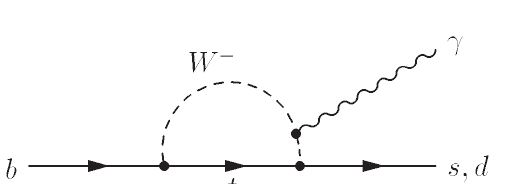
\includegraphics[width=8cm]{em_peng.JPG}
\caption{\label{fig:Btosd_fcnc}
The electromagnetic penguin diagram \cite{Lingel:1998fa}.}
\end{figure}
The figure \ref{fig:Btosd_fcnc} shows that the $b\rightarrow s,d \gamma$ transition is a loop suppressed process. In the SM there exist no tree level diagrams for these FCNC transitions. 
\subsection{GIM mechanism}\label{GIM}
The suppression of the $b\to s(d)$ was further explained by the Glashow-Illiopoulos-Maiani (GIM) mechanism. The amplitude of figure \ref{fig:Btosd_fcnc} is given by \cite{Grinstein:2017pvg}
\begin{eqnarray}
\mathcal{M}=e q_{\mu} \epsilon_{\nu} \bar{u}\left(p_{s}\right) \sigma^{\mu \nu}\left(\frac{1+\gamma_{5}}{2}\right) u\left(p_{b}\right) \frac{m_{b}}{M_{W}^{2}} \frac{g^{2}}{16 \pi^{2}} \cdot I,
\end{eqnarray}
where 
\begin{eqnarray}\label{btos_amp_factor}
I=\sum_{i=u, c, t} V_{i b} V_{i s}^{*} F\left(\frac{m_{i}^{2}}{M_{W}^{2}}\right).
\end{eqnarray}
The term $\frac{g^2}{16\pi^2}$ is a loop factor, and it can be given as $\frac{g^{2}}{16 \pi^{2}} \sim \frac{\alpha}{4 \pi \cos^2\theta_{W}}$. We insert the $b$ quark mass $m_b$ to flip the chirality of the $b$ quark.\par
In equation (\ref{btos_amp_factor}), the function $F(x)$ arises by the explicit calculation of the diagram. Since $m_t\gg M_W$, we cannot safely Taylor expand the function $F(m_i/M_W)$. The function $I$ is invariant under $F(x)\to F(x)+ \mbox{constant}$ from the unitarity of the CKM matrix. Under this transformation $F(0)=0$ without loss of generality. Besides, the unitarity of the CKM matrix elements provide $V_{t b} V_{t s}^{*}=-\sum_{i=u, c} V_{i b} V_{i s}^{*}$. Following from this, we obtain
\begin{eqnarray}
I=-V_{c b} V_{c s}^{*}\left(F\left(\frac{m_{t}^{2}}{M_{W}^{2}}\right)-F(\frac{m_{c}^{2}}{M_{W}^{2}}) \right)-V_{u b} V_{u s}^{*}\left(F\left(\frac{m_{t}^{2}}{M_{W}^{2}}\right)-F(\frac{m_{u}^{2}}{M_{W}^{2}}) \right).
\end{eqnarray}
Since $m_u, m_c\ll M_W$, the term $F(m_{u,c}^2/M_W^2)$ can be expanded in Taylor series. This gives
\begin{eqnarray}
\begin{aligned}
I &=-V_{c b} V_{c s}^{*}\left(F\left(\frac{m_{t}^{2}}{M_{W}^{2}}\right)-F^{\prime}(0) \frac{m_{c}^{2}}{M_{W}^{2}}\right)-V_{u b} V_{u s}^{*}\left(F\left(\frac{m_{t}^{2}}{M_{W}^{2}}\right)-F^{\prime}(0) \frac{m_{u}^{2}}{M_{W}^{2}}\right)+\cdots \\
&=F\left(\frac{m_{t}^{2}}{M_{W}^{2}}\right) V_{t b} V_{t s}^{*}+F^{\prime}(0) \sum_{i=u, c} V_{i b} V_{i s}^{*} \frac{m_{i}^{2}}{M_{W}^{2}}+\cdots \\
& \sim \epsilon^{2} F\left(\frac{m_{t}^{2}}{M_{W}^{2}}\right),
\end{aligned}
\end{eqnarray}
where $\epsilon^{2}=A\lambda^2$ in the Wolfenstein parameterization. The combination of loop suppression, mass suppression and CKM suppression is provided by GIM mechanism. As a result, the FCNC are highly suppressed in the SM. Also, the contribution from $F(m_u^2/M_W^2)$ and $F(m_c^2/M_W^2)$ is negligible compared to the $F(m_t^2/M_W^2)$. Thus, the virtual top quark exchanges dominate the $b\to s(d)$ amplitude.
\subsection{Effective weak interactions}
In the SM, the coupling of the $W^{\pm}$ bosons to the fermions are the only flavor changing interactions \cite{Neubert:2005mu}. At low energies, i.e. $E\ll M_W$, we can ignore the effects of the heavy bosons. This is known as integrating out of the heavy degrees of freedom (see sec \ref{sec:HQET}). As a result, a full SM interaction is converted into a local four fermion interaction. The effective Lagrangian can be expressed by a series of effective vertices and their effective coupling constants (see sec \ref{section:OPE_b}). These \textit{effective coupling} constants provide the short distant (high energy) physics, and they are known as Wilson coefficients ($C_i$). The long distant (low energy) physics is given by effective operators $\langle Q_i \rangle$. Since the Wilson coefficients are associated with high energy scales, where $\frac{\alpha_s}{\pi}\sim 0.1$, they can be perturbatively expanded in $\alpha_s$. This is because at high energy scales the $C_i$ are obtained by matching the effective diagrams with the full theory diagrams at the weak scale ($\mu\sim M_W$). For example, the explicit form of the first two Wilson coefficients are \cite{Neubert:2005mu}
\begin{eqnarray}\label{C1C2_will_co}
\begin{array}{l}
C_{1}(\mu)=1+\frac{3}{N_{c}} \frac{\alpha_{s}(\mu)}{4 \pi}\left(\ln \frac{M_{W}^{2}}{\mu^{2}}-\frac{11}{6}\right)+O\left(\alpha_{s}^{2}\right) \\
C_{2}(\mu)=-3 \frac{\alpha_{s}(\mu)}{4 \pi}\left(\ln \frac{M_{W}^{2}}{\mu^{2}}-\frac{11}{6}\right)+O\left(\alpha_{s}^{2}\right)
\end{array}
\end{eqnarray}
In equation (\ref{C1C2_will_co}) $C_1$ and $C_2$ are expanded in terms of $\frac{\alpha_{s}}{\pi} \ln \frac{M_{W}^{2}}{\mu^{2}}$ instead of $\frac{\alpha_s}{\pi}$. The $\frac{\alpha_{s}}{\pi} \ln \frac{M_{W}^{2}}{\mu^{2}}\sim 0.8$. These large logarithmic terms needs to resummed to all orders.\par
The solution to the problem of large logarithms is by using renormalization-group (RG) improved perturbation theory. It treats $\alpha_{s} \ln \frac{M}{\mu}$ as $\mathcal{O}(1)$ and $\alpha_s\ll 1$. In appendix A we provide the RG evaluation of the dominant Wilson coefficients of $\bar{B}\to X_s \gamma$. 